

\documentclass[11pt, a4paper]{article}
\usepackage{wrapfig}
\usepackage{fancyhdr} 
\usepackage[a4paper, left=2cm,right=2cm,top=2cm,bottom=1.5cm]{geometry}
\usepackage{appendix}
\usepackage{graphicx} % Required for inserting images
\graphicspath{ Figures }
\usepackage{amsmath}
\usepackage{comment}
\usepackage{amsfonts}
\usepackage{booktabs}
\usepackage{hyperref}
\usepackage{siunitx}
\usepackage{fancyhdr}
\usepackage{algorithm}
\usepackage{algpseudocode}
\usepackage{dsfont}
\usepackage{cuted}
\usepackage{booktabs}
\usepackage{multirow}
\usepackage{tabularx}
\usepackage{listings}
\usepackage[dvipsnames]{xcolor}
\usepackage{sectsty}
\usepackage{pdfpages}
\definecolor{section_heading}{RGB}{0, 59, 113}
\sectionfont{\color{section_heading}}  
\subsectionfont{\color{section_heading}}  
\subsubsectionfont{\color{section_heading}}  
\paragraphfont{\color{section_heading}}  
%\usepackage{svg}
\usepackage{array}
\usepackage{colortbl}
\usepackage{multirow}
\usepackage{multicol}
\usepackage{placeins}
\usepackage{makecell}
\usepackage{parskip} 
\usepackage[inkscapearea=page]{svg}
\svgsetup{inkscapeexe={~/inkscape-wrapper.sh}}
\lstdefinelanguage{OpenCL}{
	language=C,
	morekeywords={__kernel, __global, __local, __constant, __private,
		kernel, global, local, constant, private,
		get_global_id, get_local_id, get_group_id,
		get_global_size, get_local_size, get_num_groups,
		barrier, CLK_LOCAL_MEM_FENCE, CLK_GLOBAL_MEM_FENCE,
		float2, float3, float4, float8, float16,
		int2, int3, int4, int8, int16,
		uint2, uint3, uint4, uint8, uint16,
		char2, char3, char4, char8, char16,
		uchar2, uchar3, uchar4, uchar8, uchar16,
		image2d_t, image3d_t, sampler_t,
		read_imagef, write_imagef, read_imagei, write_imagei},
}
\lstset{
	%language=OpenCL,
	basicstyle=\ttfamily\footnotesize,
	keywordstyle=\color{red}\bfseries,
	commentstyle=\color{green!50!black}\itshape,
	stringstyle=\color{orange},
	morekeywords={size_t, cl_int, cl_uint, cl_float, cl_double, cl_bool, cl_kernel, cl_mem, queue, kernel, enqueueNDRangeKernel, NullRange, NDRange},
	literate=
	{0}{{\textcolor{orange}{0}}}{1}
	{1}{{\textcolor{orange}{1}}}{1}
	{2}{{\textcolor{orange}{2}}}{1}
	{3}{{\textcolor{orange}{3}}}{1}
	{4}{{\textcolor{orange}{4}}}{1}
	{5}{{\textcolor{orange}{5}}}{1}
	{6}{{\textcolor{orange}{6}}}{1}
	{7}{{\textcolor{orange}{7}}}{1}
	{8}{{\textcolor{orange}{8}}}{1}
	{9}{{\textcolor{orange}{9}}}{1},
	numbers=left,
	numberstyle=\tiny\color{gray}\ttfamily,
	numbersep=10pt,
	breaklines=true,
	showstringspaces=false,
	backgroundcolor=\color{gray!12},
	frame=single,
	frameround=tttt,
	rulecolor=\color{gray!30},
	xleftmargin=15pt,
	framexleftmargin=15pt,
	aboveskip=10pt,
	belowskip=10pt,
	columns=fullflexible,
	keepspaces=true,
	%identifierstyle=\color{black!80},  % slightly grey identifiers
	emphstyle=\color{cyan},
}
\usepackage[
    style=ieee,
    sorting=none,
    citestyle=numeric-comp,
    backend=bibtex,
    doi=false,
    isbn=false,
    url=false,
    eprint=false
]{biblatex}

\AtEveryBibitem{
    \clearfield{urlyear}
    \clearfield{urlmonth}
    \clearfield{urlday}
}

\addbibresource{refs.bib}
\usepackage{amsmath,amsthm,amssymb,setspace,enumitem,epsfig,titlesec,verbatim,color,array,eurosym,multirow,blkarray,lscape,soul,graphicx,comment,nicefrac,lineno,epstopdf,accents,pifont}
\usepackage[bf,small]{caption}
\DeclareMathSizes{11.5}{20}{14}{10}   % For size 11 text
\renewcommand{\headrulewidth}{0pt}
\renewcommand{\qedsymbol}{$\hfill\blacksquare$}
\hypersetup{
	colorlinks=true,
	linkcolor=black,
	citecolor=blue,
	urlcolor=blue,
	filecolor=black
}

\newcommand{\refeq}[1]{\hyperref[#1]{Equation \ref{#1}}}
\newcommand{\reffig}[1]{\hyperref[#1]{Figure \ref{#1}}}
\newcommand{\reftbl}[1]{\hyperref[#1]{Table \ref{#1}}}
\newcommand{\refapn}[1]{\hyperref[#1]{Appendix \ref{#1}}}
\newcommand{\refsec}[1]{\hyperref[#1]{Section \ref{#1}}}
\newcommand{\reflst}[1]{\hyperref[#1]{Listing \ref{#1}}}
\newcommand{\refalg}[1]{\hyperref[#1]{Algorithm \ref{#1}}}
\newcommand{\refsup}[1]{\hyperref[#1]{Supplementary Material}}

\usepackage{caption}
\usepackage{subcaption}

\title{FPGA-based mix-precision Monte Carlo using high level synthesis tools}
\date{
	EGH490-1 Project Proposal\\
	\vspace{10mm}
	October 23, 2026
}
\pagestyle{fancy}
\fancyhf{} 
% Footer config
\fancyfoot[C]{\raisebox{0.2cm}{\thepage}}
\fancyfoot[L]{
\includegraphics[height=0.75cm]{Figures/Misc/QUT_logo_footer.png}} 
\fancyfoot[R]{\raisebox{0.2cm}{L. Lubrano Lavadera}}
\fancyhead{} 
\renewcommand{\headrulewidth}{0pt} 
\renewcommand{\footrulewidth}{0.4pt}

\begin{document}
	\maketitle
    \pagenumbering{Roman}
    \vspace{200px}
    \begin{center}
        Author:\\
        \vspace{0.4cm}
        \textbf{{\Large Luca Lubrano Lavadera}}\\
        \vspace{0.8cm}
        Under the supervision of:\\
        \vspace{0.4cm}
        \textbf{{\Large Dr Jasmine Banks}}\\
        \vspace{0.4cm}
        \textbf{{\Large Dr David J. Warne}}
    \end{center}
    \vfill
    \begin{figure}[h!]
        \centering
        
\includegraphics[width=0.3\linewidth]{Figures/Misc/QUT-logo.png}
    \end{figure}
    \thispagestyle{empty}
    \newpage
    \tableofcontents
    \newpage
    \listoffigures
    \listoftables
    \newpage
    \hypersetup{
    	colorlinks=true,
    	linkcolor=blue,
    	citecolor=blue,
    	urlcolor=blue,
    	filecolor=black
    }
    \pagenumbering{arabic} 
	
	\section{Introduction}
	Most fields in modern engineering depend heavily on data intensive high performance computing (HPC). Server-based computation, such as data-centres and computational research facilities, are estimated to have produced more greenhouse gas emissions than the aviation sector in 2020 \hl{cite}. The impact of this has only increased with the rise in popularity of machine learning tools, such as artificial intelligence (AI), within the field \hl{cite}. Many of these computationally burdensome tasks require the parallelism of time-series simulations, such as Finite Element Analysis (FEA) and Stochastic simulation --- used in AI applications heavily \hl{cite}. 
	
	But as methods become more complex, and problems more difficult, it is infeasible to simply continuously add more computational devices to a cluster. This presents several types of issues, perhaps the most serious of which is the power input required to operate supercomputers. GPU-dense heterogeneous computing environments, used extensively in engineering modelling and simulation, dissipate \hl{enormous} amounts of heat which utilises a substantial quantity of power to cool. From this, GreenHPC aims to increase the amount of floating-point operations per second per watt (FLOPS/W) --- unlike traditional HPC, which is solely concerned with the FLOPS --- leveraging of specialised computing devices such as, tensor processing units (TPUs), application-specific integrated circuits (ASICs) and field programmable gate arrays (FPGAs). 
	
	Clearly, the most power-efficient computational devices are ASICs, since they are purpose-built to perform operations at the circuit level. While this is useful in large supercomputers that perform extremely repetitive low-variant tasks, it is applicable to computational research. Reconfigurable computing however, positions itself to improve upon some of these flaws, by allowing the user to achieve \textit{near} true-circuit throughput efficiency while allowing for modifications to be made. These devices, primarily FPGAs, have been extensively used in the Electrical Engineering field for printed circuit board (PCB) design and have recently gained significant popularity in computational settings. 
	
	Unfortunately however, the tools available to develop softrware on these devices has been, until recently, extremely niche with specialisation in electrical circuit design essentially being a pre-requisite. Recent developments in compilation tool chains have now reduced this barrier to entry. With the extension of portable programming frameworks, such as OpenCL and HIP, to now be able to target not only CPU/GPU infrastructure but also FPGAs. This significantly reduces the development overhead as well as the skill barrier, as these frameworks are almost exclusively variations to C/C++ --- industry standard for computational research.
	
	To examine how these competing goals of increased throughput and reduced power-consumption can be evolved by the use of reconfigurable hardware in heterogeneous computing environments, we consider implementations of parallelisable stochastic processes for inference. These time-series, non-deterministic processes are representative of many advanced engineering simulations in fluid-flow and are the next challenge in implementation for reconfigurable devices. 

	\subsection{Research Questions}
	The aim of this work is to understand how reconfigurable computing can be used to compilment highly heterogeneous computing environments via reduction in total heat dissipation, hence reducing total power consumption. We investigate the following research questions to this end.
	\begin{enumerate}
		\item To what extent can implementations of mixed-precision Monte Carlo on reconfigurable computing hardware improve the power efficiency of algorithms compared to graphical processing units?
		\item To what extent can high-level synthesis tools and portable code frameworks be used to reduce the development time of algorithms in heterogeneous computing environments?
	\end{enumerate}
	
	\subsection{Contribution}
	The core expected contribution of this work is the implementation and analysis of novel simulation techniques utilising reconfigurable hardware. This is done through the portable programming framework, High-level Synthesis (HLS), which uses pragmatic flagging of \hl{standard} C++ code. Due to the size and complexity of this task, we segment our deliverables into clear milestones to enable clear progress throughout the project. The contribution delivered in EGH490--1 is the validation of the implementation of methods of simulated FPGA hardware --- evaluated against GPU-based implementations. With the physical FPGA hardware testing and analysis against existing methods being done in EGH490--2.

	\section{Interim Deliverables}
	We divide this project into two key aspects, first is the development of simulation algorithms and validating their outputs against proven methods using hardware emulation. Since, this involves both the understanding of heterogeneous computing code architectures and the specific methods in which the HLS compiler converts C++ to hardware description language (HDL). Following from this, we intend to undertake extensive power utilisation studies on the target FPGA cluster on the QUT supercomputer, \textit{Aqua}. This process involves the compilation of high board utilisation code and as such will take in the order of hours per experiment, meaning the initial validation and verification analysis we conduct in this initial report is vital for the proceeding work.
	
	\subsection{Codebase}
	This project entirely revolves around the development of a codebase \textit{case study} of how reconfigurable computing devices can be used in heterogeneous computing. As such, we construct a well structured and properly documented codebase to support both the claims we make within this, and future, work and provide a framework to those who may wish to implement similar systems. The codebase can be found under \hyperlink{https://github.com/LucaLubrano/fpga-hls-codebase}{FPGA HLS Codebase}.
	
	The first major component to the codebase is the custom kernel library. These kernels are the pieces of code that are compiled --- through some intermediaries --- to bitstream\footnote{A set of binary configuration instructions loaded on the FPGA when performing computations that the cards runtime, XRT, uses to program the physical hardware.} and are how we interact with the FPGA. The programmatic structure of these kernels can be related heavily to that of GPU-based kernels which are already widely used and understood in computational applications. However, unlike these implementations, the FPGA, and reconfigurable computing in general, does not have the same clear path of program and data flow as these static devices. We instead utilise the \texttt{pragma} preprocessor directives to instruct the compiler as to the specific hardware configuration we desire. 
	
	Significant time was spent in order to be able to produce meaningful simulation results using this framework. while predominantly the simulation logic itself is written in C++14, the majority of the complexity comes from the data parcing to and from the host, CPU, and device, FPGA. The host code was written utilising the OpenCL\footnote{An open-sourced coding standard based on C specialised for cross-vendor heterogeneous computing environments. It allows for host code to execute parallel computing kernels on varying compute device archictectures with minimal change and standardised memory hierarchy.} standard. This is relevant to our research as one of the key goals is to determine whether the time investment in utilising reconfigurable hardware is achievable for scientific researchers. Having the ability to develop standardised host code across compute devices, only having to develop specialised kernel code, could significantly increase the viability of such a solution. 
	
	\begin{figure}[h!]
		\centering
		\rule{0.8\textwidth}{8cm} 
		\caption{Visualisation of the simplified structure of a field programmable gate array.}
		\label{fig:fpga_internals}
	\end{figure}
	
	When developing the FPGA kernels, it is important to understand how the device is indeed reconfigurable as this affects the structuring and pragmatic flagging of the kernel. Since essentially, when we load a kernel onto the FPGA, we are consuming \textit{space} on the device, we optimise our kernels to be physically compact such that we can load as many as possible onto the card. This is how we achieve the parallelism of our simulation similar to the operation of a GPU. \reffig{fig:fpga_internals} describes the general high-level structure of the card, \hl{come back to}

	The compilation of kernel code to an instruction set that is able to be utilised by the FPGA is a cascading process. \hl{add to} 
	\begin{figure}[h!]
		\centering
		\rule{0.8\textwidth}{8cm} 
		\caption{Visualisation of the compilation and execution of code on a supercomputer using field programmable gate arrays. \hl{HLS C++ code $\rightarrow$ system linking $\rightarrow$ logic synthesis $\rightarrow$ routing $\rightarrow$ bitstream generation --- describe the processes the user is involved with and what is handled by the compiler}}
		\label{fig:kernel_loading}
	\end{figure}
	
	\subsection{Preliminary Studies}
	To demonstrate the performance of our codebase, we utilise biochemical reaction networks (BCRNs) as a case study. The mathematical modelling of biological process is a computational expensive task and is well suited to heterogeneous computing environments. The specific choice of simulation is not of particular relevance, however, this example demonstrates the kind of behaviour that would benefit from an optimisation process. The internal workings of the simulation itself are not parallelisable, since it relies on previous time data --- common in fluid flow modelling as well --- but is parallelisable amongst indepedent simulations. This is critical, especially in inference-based problems, such as those faced by AI development, as enormous amounts of simulations are required to provide accurate outcomes.
	
	\subsubsection{Biochemical Reaction Networks}
	We begin by focusing on simple production degredation reaction networks that are well studied and can be verified by existing code. This allows us to check the validity of algorithms on the FPGA, as well as provide a performance benchmark that will be used in later work to understand runtime and power efficiency changes between devices. Further to this, the compilation of complex kernels from HLS to FPGA instruction set requires a non-zero computational time, in the order of tens of hours for larger kernels. By choosing a low species, and setting a low initial population, we increase our ability to rapidly experiment and validate our methods. 
	
	\begin{figure}[h!]
		\centering
		\rule{0.8\textwidth}{8cm} 
		\caption{Monomolecular chain model for the production and degredation of two molecules.}
		\label{fig:mmc_process}
	\end{figure}
	The exact system we use is the Monomolecular Chain (MMC) model, described in \reffig{fig:mmc_process}. This model describes the production of molecular A from an external environment, the decay of molecule A to molecule B, and the external consumption of molecular B. The exact solution for the behaviour of the population to this model can indeed be solved analytically using the chemical master equation \hl{cite}. We do not conduct this analysis in this work, however, this is a secondary method we are able to use to verify the integrity of our methods. Noting in \reffig{fig:mmc_process} the $k$ parameters represent the rate in which the three different reactions occur. 
	
	\subsubsection{Euler-Maruyama Simulation}
	To model the stochastic processes involved in biochemical reaction network modelling, we use stochastic simulation algorithms (SSA). There are many popular and well-studied methods to implement these algorithms, broken into two main catagories; exact\footnote{An exact solution means the algorithm computes an exact realisation of the chemical master equation to find the solution at the next timestep.} and approximate\footnote{An approximate algorithm encompasses many different algorithms which each utilise discretisations of the governing stochastic equations to progress the solution.} solutions. We select the Euler-Maruyama algorithm, an approximate SSA, which discretises the Ito stochastic partial differential equation representation of the chemical Langevin equation. This algorithm is widely used in the literature as a standard method for solving these systems, and also exhibits preferable programmatic characteristics. \reffig{fig:example_simulation} shows an example realisation of the Monomolecular chain model using the Euler-Maruyama algorithm.
	
	\begin{figure}[h!]
		\centering
		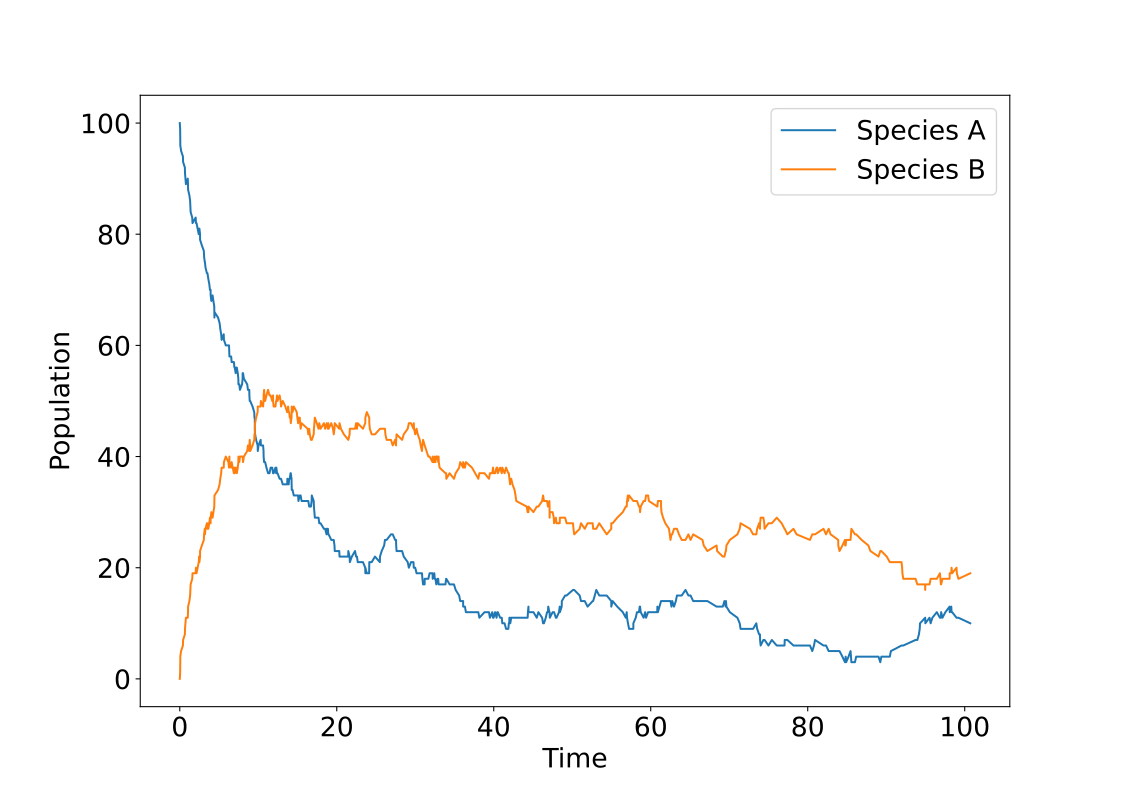
\includegraphics[width=0.75\textwidth]{Figures/mmc-gdm-example-samplepath.png} 
		\caption{Example Euler-Maruyama method sample path of the Monomolecular chain model using C++ on a
			GPU. With kinetic rate parameters $k_1 = 1.0$, $k_2 = 0.1$ and $k_3 = 0.05$, initial conditions $A(0) = 100$, $B(0) = 0$, final time $T = 100$.}
		\label{fig:example_simulation}
	\end{figure}
	In this type of simulation, it is well-known that the predominant computational cost arise from the generation of random numbers. Additionally, we also require these random numbers to be distributed, which necessitates expensive mathematical operations. Since, each SSA requires a distributed random number per species per time-step incrementation, significant focus is often placed in understanding how we can increase the efficiency of this operation to increase the efficiency of the overall algorithm. Since the Euler-Maruyama method only requires unit Normal random numbers, we can infact simply generate uniform random numbers and transform them to Normals via the Box-Muller transform \hl{cite}. The process of random number generation on reconfigurable hardware is explored further in \refsec{sec:future_work}.
	
	\subsection{Initial Findings}
	
	
	\subsubsection{Hardware Emulation}
	
	\begin{figure}[h!]
		\centering
		\rule{0.8\textwidth}{8cm} 
		\caption{vivado analysis.}
		\label{fig:vivado_analysis}
	\end{figure}
	
	\begin{figure}[h!]
		\centering
		\rule{0.8\textwidth}{8cm} 
		\caption{fpga utilisation.}
		\label{fig:fpga_utilisation}
	\end{figure}
	
	\subsubsection{Validation of Implementation}
	\begin{figure}[h!]
		\centering
		\rule{0.8\textwidth}{8cm} 
		\caption{overlayed plot.}
		\label{fig:comparison}
	\end{figure}
	
	\begin{figure}[h!]
		\centering
		\rule{0.8\textwidth}{8cm} 
		\caption{mean behaviour.}
		\label{fig:mean_behaviour}
	\end{figure}
	
	\subsubsection{Physical Hardware}
	Within the scope of this interim deliverable report, we aimed to produce preliminary results mainly on emulated FPGA hardware. This was due to identified risks in our project proposal surrounding access to FPGA hardware on the QUT HPC. Through discussion between the academic supervisors and the DevOps team at the QUT HPC, the hardware was not able to be configured in a timeframe that aligned with this project. However, through continued conversation with the DevOps team, we were able to organise the validation of FPGA hardware on the HPC via job-queueing. This meant that all necessary toolchains were loaded we were able to compile and execute example FPGA kernels on the FPGA cluster. 
	
	This is a key milestone in the ability to conduct the second phase of the proposed research moving into the second semester. While the FPGA cluster is still not fully matured for general use, it is in a state that we are able to develop our algorithms within. Including the compilation and execution of our emulated algorithms on physical hardware, which will lead into much of the analysis to be completed in future work, see \refsec{sec:future_work}.
	
	\section{Risk Management}
	Risk management is an important tool utilised through the entire duration of the project and will be continued to be used in the next section of work. Due to the interdependant nature of this project to different groups within QUT, and the necessity of the operation of specific hardware, we have developed several contingency approaches to ensure progress can always be made. This is done through the initial development and verification of algorithms using hardware emulation. Allowing progress to be made while coordinating with the HPC DevOps team to allow access for the FPGA cluster. This was not able to be achieved in the provided timeframe of this project and will fall into objectives to be completed in the second part of this research.
	
	\subsection{Health \& Safety}
	We update the risk assessment initially created at the beginning of this report to encapsulate identified risks and hazards, and their corresponding mitigations, see \refapn{apn:RA}. To date, there have been no incidents or near misses in relation to this project. We continue to ensure that health and safety standards are upheld during the project duration and monitor the risks reported in the risk assessment. 
	
	\subsection{Progress Inhibitors}
	Progress inhibitors refer to areas of the project that stopped the ability of other parts of the project to be completed. Due to the nature of the hardware, and associated software pipelines, that we used in this project, licensing was an issue through the beginning of the project. This halted progress in the validation and verification of some early aspects of the project, pushing this back and altering the deliverable timeline. This was resolved through collaboration with the supervisors to find appropriate methods for obtaining licensing through the QUT system. Secondly, was access to the QUT HPC FPGA cluster which is discussed elsewhere in the report, however, was resolved with the collaboration with the QUT HPC DevOps team to set this resource up for open access utilisation. 
	
	\subsection{Emergent Issues}
	In completing the first section of work for this project, issues that may hinder the ability to make progress in the second phase of the research are more visible. Compilation time of simulation kernels is a problem that was thought to be an issue when presenting the project proposal, and has been confirmed to require a significant time investment. This was done during the early validation of the FPGA cluster software installation done on the HPC. We plan to mitigate this risk in project planning and methodology, since our much of our works will be studies on utilisation and efficiency. Meaning we should be able to store and reuse many of the kernel compilations we conduct, given our algorithms are already validation on emulated hardware. 
	
	A secondary issue that we anticipate to impact the project is the isolation of resources on the HPC to be able to conduct in-depth studies. The primary objective of the first section of work was to research, develop and experimentally validate algorithms. We know wish to move to hardware implementations and understand how power utilisation and efficiency scale with FPGAs as compared to GPUs. In order to conduct this study with integrity, we need to be able to isolate the power utilisation and card utilisation of the targetted FPGA and GPU clusters. This is not something that is clearly stated when scheduling jobs with the HPC and may require an amount of custom setup or node modification. We plan to develop a method for conducting this study in heavy collaboration with DevOps team. 
	
	\section{Ethics}
	Within this project, we strive to uphold the core values and principles describe by Engineers Australia; demonstrating integrity, practising competently, exercising leadership, and promoting sustainability. When conducting all research in this project, we at all times demonstrate integrity when comparing algorithms, collecting data, and crediting work. To ensure that the comparisons we make are fair, we utilise implementations of algorithms developed in previous work that closely follow the structure of the algorithms used here --- for GPUs. Meaning that when we benchmark the results between both the FPGA and GPU, we are analysing comparable data, and not skewing results. 
	
	We demonstrate competence through our work ensuring the methodology we conduct is reviewed by the academic supervisors. Furthermore, we acknowledge the limitations in knowledge when conducting experimentation and optimisation throughout honestly. Some areas of the codebase may not be strictly optimised equivalently between the two implementations. However, we aim to showcase how a scientific researcher may use this tool, and as such, deem this to be acceptable.
	
	Leadership is shown expressly when communicating to the DevOps team at HPC. Leading the finalisation of the creation of the FPGA cluster on the HPC. This involved several months of communication with the HPC team and conducting investigations independantly to assist the team. We also ensure to not make erroneous claims within this work before understanding the full picture of the work. Given this is a preliminary report we are not able to make definitive claims about the results of our findings and ensure to clearly state the limitations to our approach.
	
	\subsection{Sustainability}\label{sec:sustainability}
	Sustainability has been a focus and forms a key part of our overall research goal. The largest risk to sustainable practice in our work is the efficiency gained is offset by energy development costs of methods \hl{cite}. To reduce the impact of the development and experimentation that we complete in this work, we spend significant time ensuring that our algorithms are validated in emulation before moving to hardware. The computational cost for developing in emulation is significantly less than that of hardware and allows us to validate the correctness of our solution without requiring the large computational time required to run on the actual FPGA. Meaning, that when we move to hardware implementations we are already confident in our implementation. By doing this, we both significantly increase our efficiency in developing algorithms, as code-to-test time is reduced, and the overall power use of our research. 
	
	Another sustainability risk that has been examined throughout our research is Jevon's Paradox, by which efficiency is offset by greater consumption. The rise of artificial intelligence is a clear follower of this paradox, as computational power has only exponentially increased, and yet the demand and consumption of these models has also increased. In the scope of our work, by decreasing the total cost of simulation in a biochemical reaction network context, the long-term goal is to reduce the wall-time and power utilisation in inference problems. Complex inference problems often requires in the magnitude of days and weeks worth of computational time on a supercomputer. The goal criterion of the analysis however, does not often change. As such, increasing the throughput ability is aimed to not increase total demand. 
	
	\section{Project Collaboration}
	The main line of development work done in this report has been mostly completed individually. Since, the scope of this interim deliverable has been the development of the kernels themselves to be later used in studies, strong project collaboration was not critical to the completion of this scope of works. However, in the organisation of resources and the looking forward to the goals of the overall project, collaboration will be critical to meet milestone deadlines. This project, and the work conducted within, are research based, meaning we have not engaged an industry partners.
	
	\subsection{Stakeholders}
	There are three main stakeholder groups that we consider in this work. The first of which being the supervisors involved in the project proposal and ideation. Both supervisors utilise large computational models for analysis in their relevant fields of research, Electrical Engineering and Computational Mathematics. As such, they have a vested interest in the success of the project and have been key in the progress of several aspects of the research, especially in interfacing to other university departments for things such as licensing and hardware access. 
	
	Another significant stakeholder to the project is the QUT HPC DevOps team. This group is responsible for the on going improvement and development of the supercomputer, Aqua. Through collaboration with them, we have been able to assist in pushing for the opening of the FPGA cluster, which until this project remained inaccessible to researchers. By showing that this a resource that can be utilised by researchers we can assist this team in more fully utilising the supercomputer as well as potentially demonstrate an avenue they can utilise to reduce power consumption on the HPC for large parallelisable computational tasks. 
	
	The final stakeholder we consider are the potential end-users of our programs and methodologies. Our target is scientists who utilise HPC environments for computationally intensive research. Throughout the research we consider the complexity of the code and results we produce to ensure that we provide a fair analysis as to whether HLS is accessible to this group of researchers who are potentially not trained in computer science or do not have the time to implement such methods. 
	
	\subsection{Resources}
	The primary resources used in the codebase developed were the OpenCL and HLS coding standards \hl{cite}. These provided the necessary documentation and explanation of concepts to be able to create compliant code. In parallel to this we heavily utilised open sourced example repositories provided by AMD for their HLS codebase and FPGA development pipelines \hl{cite}. These repositories, alongside the documentation, allow us to create code that is efficient and follows the intended structure to reduce potential issues or overheads.
	
	To complete the next milestone deliverable, we will also utilise the AMD U55C FPGA card located in the QUT HPC. We will draw upon the guidance of the DevOps team and the appropriate documentation for implementing programs on this hardware. Since this can be a quite difficult and ownersome task we will ensure to collaborate heavily with the academic resources available to reduce delays to the project. 
	
	\section{Discussion}
	The proposed methods that we have implemented show viability to be implemented on FPGA hardware through preliminary studies. We are able to simulate on emulated hardware, which represents a close software twin of the physical device. We anticipate that the results observed in the emulation will closely reflect the true behaviour of the FPGA and as such can be used as a preliminary validation of algorithms. This positions the work well to move into the second phase of deliverables and conduct hardware case studies in power utilisation and wall-time. 
	
	Through the implementation of a OpenCL framework, we reduce the overhead introduced by the addition of the FPGA into our compute cluster. The HLS kernel code compiles seperately to our main portable code base and as such can be easily configured within the host code to be used. This ability to utilise portable algorithms allow us to have standardised that contains the pre and post processing of data, with the simulations being conducted on any OpenCL supported hardware. This significantly reduces the time investment of researchers in developing their codebases to include FPGA hardware as the only \textit{unique} component is the FPGA kernel itself. Meaning the same codebase can be used on CPUs, GPUs, and FPGAs with minimal change depending on available resources, making it a more attractive solution. 
	
	\subsection{Future Work}\label{sec:future_work}
	There are several key avenues we wish to extend this work towards to gain a better understanding of how FPGA accelerator cards can be integrated into scientific research. The logical first step to proceeding will be to validation our algorithms on the physical FPGA hardware now that we have access to the cluster. We then wish to understand how the wall time of simulations differs from a GPU to an FPGA. This will give us a preliminary understanding of how efficient the FPGA is for simulation. A critical complexity will also be to understand how the power consumption changes between a GPU and an FPGA implementation. This will involve work with the HPC in determining total overhead cooling power usage and will require heavily collaboration with the QUT HPC teams. We will also monitor and report on the complexity of moving from a GPU codebase to an FPGA codebase, in all aspects, including; code complexity, process complexity, and general usage complexity. This will give us a picture of how this hardware can fit into existing and new computational research methods. 
	
	\paragraph{Timing Studies}
	By conducting a wall time study on our FPGA algorithms, and comparing to existing GPU implementations, we hope to understand the relative performance on the hardware. While this will not give us an answer on whether the hardware is more power efficient for this use case, it will answer a key question of run time scaling. Since, many computational researchers require their simulations to run within specific timeframes and under specific budget, both monetary and computational, this will allow us to begin to answer hte usability question posed. 
	
	We intend to conduct this timing study utilising primarily the diagnostic tools provided by the AMD HLS software development pipeline in Vivado Vitis. In our preliminary investigations of emulated software, we attempted to use a similar debug tool to understand runtime, however, had issues as the emulation does not provide true results in this respect. Since GPU implementations are already efficient, we will normalise the runtime against 100,000 simulations which allows us to see perceptible differences in performance. We will also conduct studies with varied initial conditions to ensure that we provide honest results and comparisons.
	
	\paragraph{Power Studies}
	The power study represents the key gap posed within our research questions. It also presents one of the most difficult pieces of the software to quanitfy. Under ideal conditions, we wish to experiment with how the power usage of the GPU and FPGA change under simulation load as well as under no load. This would encompass all related power usages as well, most importantly the cooling requirements for the hardware. As one of the most power inefficient components of large, GPU-dense, computing environments is the power draw resulting from cooling. 
	
	To conduct this study, we plan to isolate a small GPU cluster and run it at full utilisation to understand the total power draw, using a physical power measuring device. For initial results we would look to find the total power usage of the cooling equipment in the HPC and develop a fractional usage for the cluster. Since the HPC cluster only has a single U55C FPGA, held in a large computer cluster, we would do a similar experiment. Obviously however, since we already know that FPGAs generally consume less cooling power than GPUs, we would need to develop a method to more exactly understand this usage. This would need to be discussed heavily with the HPC team to find a solution, and presents one of the largest uncertaintities in the project. To mitigate this, we would begin by simply measuring total \textit{at the wall} power usage, noting the limitations. 
	
	\paragraph{Hardware Implementations}
	To understand whether it is feasible for this kind of hardware and the associated software overhead to realistically be used by scientists and researchers we will conduct a qualitative study on the complexity of the FPGA code refactoring process. This will encapsulate all aspects of the project and is developed concurrently with the main software development and analysis. By doing this, we hope to present a full picture of the potential benefits and limitations of using this level of hardware acceleration in a mainstream research context. 
	
	\newpage
	\appendix
	\section{Literature Review}
Through this literature review we aim to summarise the key methodologies in mixed-precision Monte Carlo methods in the literature that are relevant to our work. In this report we work to understand how we can utilise and exploit reconfigurable hardware with mixed-precision to take advantage of unique features in the computing architectures of FPGAs over GPUs. We perform this research within the context of Mathematical Biology in which large quantities of statistical independent simulations are required to produce meaningful results. This presents a clear use case for these methods as there is potential for both the wall-time and power efficiency improvements over conventional computing frameworks. 

\subsection{Heterogeneous Computing}\label{sec:heterogeneous_computing}
It is important to first understand heterogeneous computing as a framework to conceptualise how reconfigurable and accelerator hardware can be used to complement and improve existing computing ecosystems. Heterogeneous computing environments are those in which there are multiple different computer architectures, primarily central processing units (CPUs) and graphical processing units (GPUs). By doing this, we can allocate tasks in our program to these specific devices depending on the type of operations that are being done on them. 

This key advantage provided by conducting our computations in a heterogeneous environment allows us to optimise the choice of device based on suitability to the task \cite{macintoshImplementingEvaluatingHeterogeneous2019, warneHeterogeneousComputingApproach2016, macintoshImplementationParallelTridiagonal2016}. Meaning we are able to maximise the utilisation of hardware, which is beneficial since general purpose compute devices, such as CPUs and GPUs, carry high idle power costs. These systems often use a variety of these general purpose devices in combination with accelerator hardware, including application-specific integrated circuits (ASIC), intelligence processing units (IPU) and FPGAs \cite{cardosoChapter2Highperformance2017}. 

To maximise the clock cycle efficiency in our computing, we wish to keep our computations to the size of the floating point registers available on the target hardware. For current GPUs, this is double $64$-bit, single $32$-bit, and half $16$-bit. Working with these register sizes is critical in the efficiency of mixed-precision methods. By doing this, we can increase the throughput of our algorithm per clock cycle by using \textit{Single Instruction Multiple Data} (SIMD) operations \cite{warnePulsecoupledNeuralNetwork2014, warneSolvingTriDiagonalLinear}. 

\begin{figure}[h]
	\centering
	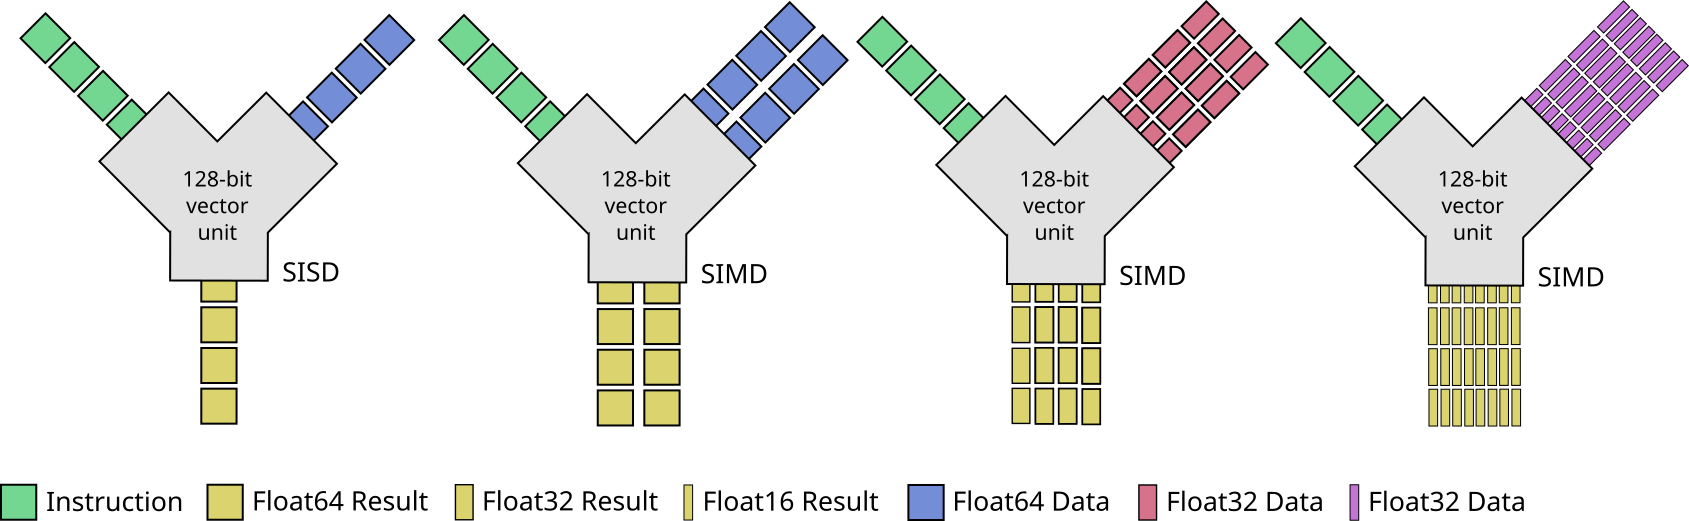
\includegraphics[width=1\textwidth]{Figures/simd.png}
	\caption{Schematic of vector unit operations in single instruction single data and single instruction multiple data configurations with varying precision levels.}
	\label{fig:simd}
\end{figure}
This works as the register is of a fixed size, usually 64-bit, each clock cycle then pushes an instruction to the register where it completes the operation on the data held. If we reduce the bit width of our data to a less precise variable type, i.e. 32 bit, the register is able to perform the same operation on two independent sets of data \cite{banksCALCULATIONENGINEPARAMETERS2014, warneComparisonHighLevel2014, deschryverFPGABasedAccelerators2015}, see diagram in \reffig{fig:simd}. Importantly, it is able to do this in the same clock cycle as if the data had been a single full precision width. This is a key part in how mixed-precision methods can provide significant speed up in high performance computing in lower precision levels \cite{warneVectorOperationsAccelerating2022}. 

Kimpson et al. \cite{kimpsonReducedPrecisionStochasticSimulation2026} investigate methods for computing simulation estimates using mixed and reduced precision in the context of stochastic simulation algorithms (SSAs). These algorithms aim to minimise the error in approximation while using native 16-bit arithmetic. At a hardware-level, this reduces the memory footprint while increasing the SIMD operations able to be computed. They specifically target GPU and tensor processing unit (TPU), which provides insight into how methods can be mapped between device hardware and the results they can achieve in heterogeneous environments. 

\subsection{Reconfigurable Computing}
Reconfigurable computing is classified by a computer architecture that is able to change its logic programming \cite{warneVectorOperationsAccelerating2022}. The most common and popular example of which are FPGAs, built from 'reconfigurable fabric' which contains the configurable logic blocks, interconnections and BRAM that allow the hardware to change its logic functions \cite{cardosoChapter2Highperformance2017}. Essentially, we can create reconfigurable circuitry at the logic-gate level, which gives the user the ability to accurately approximate the functions of a printed circuit board. 

In computing, this means that we are able to construct programs not at a software level, but instead program them onto the architecture of the card. This is a key aspect of the power efficiency that these devices can provide. Unlike CPUs and GPUs, they have a significantly reduced overhead power cost related to unnecessary and always-active processes. 

These devices have been traditionally used by electrical engineers for hardware prototyping and development, requiring users to understand low-level hardware description languages (HDLs). Hence, making them inaccessible to scientific researchers without the proper background to fully take advantage of their utility. Recent advancements in compilation software have lead to the ability for portable programming languages --- OpenCL, HLS, and others --- to be compiled into bit-stream, meaning they are now able to be used to program these devices. This has made them a target of active research in areas such as high-dimensional linear algebra \cite{warneComparisonHighLevel2014,ComparingEnergyEfficiency, macintoshImplementationParallelTridiagonal2016, macintoshImplementingEvaluatingHeterogeneous2019, warneSolvingTriDiagonalLinear}, simulation problems \cite{banksCALCULATIONENGINEPARAMETERS2014} and time-critical safety operations \cite{warnePulsecoupledNeuralNetwork2014}.

As a result of the freedom provided by FPGA hardware, we are also able to increase computational efficiency in low precision settings through the creation of unique precision levels. Unlike modern GPUs, which can provide either double (64-bit), float (32-bit) or half-precision (16-bit), we are able to define custom bit length precision data types. This can be directly applied in areas such as mixed-precision Multilevel Monte Carlo methods, which optimise the fidelity of simulations while retaining an equivalent output approximation \cite{haasNestedMLMCFramework2025}.

Intelligence processing units (IPUs) are an another emerging technology driven by the need for more specialised Artificial Intelligence computing capabilities \cite{kulkarniAcceleratingSimulationbasedInference2020}. Unlike traditional GPU architecture, which uses single-instruction multiple data (SIMD) vectorised parallelism to accelerate tasks, the IPU utilises multi-instruction multiple data (MIMD) \cite{jiaDissectingGraphcoreIPU2019}. This allows each thread to perform operations in a distinct flow, and irregular data access patterns without loss of efficiency \cite{jiaDissectingGraphcoreIPU2019}. Similarly to FPGAs, these devices are also able to define custom precision data types, which has made them extremely efficient processors in AI inference problems \cite{fitzgibbonStochasticRoundingFew2025,sunIntelligenceProcessingUnits2022,MixedPrecisionArithmeticAI}.

\subsection{Systems Biology}
To contextualise our problem we focus on the topic of systems biology, these models look to capture the complex behaviour of intracellular processes with the goal to better understand the functioning of cells as a whole \cite{abkowitzEvidenceThatHematopoiesis1996, arkinStochasticKineticAnalysis1998, kaernStochasticityGeneExpression2005, wilkinsonStochasticModellingQuantitative2009}. The classical approach to describing biological systems are continuous-time deterministic models \cite{wilkinsonStochasticModellingQuantitative2009,highamModelingSimulatingChemical2008}. Using deterministic models however, fails to explore the intrinsic randomness of biochemical reaction networks, and as such we lose valuable information about the true nature of the system \cite{elowitzStochasticGeneExpression2002,rajNatureNurtureChance2008}. As a result of this, the development of stochastic methods have become popular to capture the variability among genetically identical cells \cite{rajNatureNurtureChance2008}. 

Gene expression and regulation are fundamental applications of stochastic modelling methods in which research aims to understand the processes of cellular reproduction and phenotypic characteristics \cite{kaernStochasticityGeneExpression2005,elowitzStochasticGeneExpression2002}. It is well established that these processes are fundamentally stochastic. The nature of experimental data within whole cell modelling introduces substantial complication in generating and fitting stochastic models \cite{wilkinsonStochasticModellingQuantitative2009}. As such, it is common to instead generate stochastic simulations to produce meaningful data for analysis \cite{sunnakerApproximateBayesianComputation2013,highamModelingSimulatingChemical2008}. 

Within systems biology, a primary computational challenges is the forwards problems \cite{warneSimulationInferenceAlgorithms2019}. This refers to the prediction of future state of a system. Namely we must consider the simulation of sample paths of our biochemical reaction networks over time, and the expectation of average behaviour among all possible reaction events \cite{warneSimulationInferenceAlgorithms2019}. This is where Monte Carlo methods can be used to describe the summary statistics of the system. 

\subsection{Stochastic Simulation Algorithms}
To understand the overall behaviour of biochemical reaction networks (BCRN), we concern ourselves with only the change in population over time of the molecular species \cite{gillespieExactStochasticSimulation1977,highamModelingSimulatingChemical2008, warneSimulationInferenceAlgorithms2019, wilkinsonStochasticModellingQuantitative2009}. We consider a spatially homogeneous system for the purposes of this work \cite{chenStochasticModelingSimulation2017}. Consider a BCRN with the $N$ unique chemical species, that interact according to $M$ distinct chemical reactions. The $j^{\text{th}}$ reaction is denoted by
\begin{equation}
	\sum_{i=1}^{N} \nu_{i,j}^- X_i\rightarrow\sum_{i=1}^{N} \nu_{i,j}^+ X_i,
\end{equation}
where $\nu_{i,j}^-$ and $\nu_{i,j}^+$ are the reactant and product stoichiometries related to the $i^\text{th}$ chemical species in the $j^\text{th}$ reaction. We denote $X_i(t)$ as the copy number, that is the number of molecules in the system, of the $i^{\text{th}}$ chemical species at time $t>0$. This leads to the system state vector, $\mathbf{X}(t) = [X_1(t),...,X_n(t)]^\intercal$
In the event that the $j^\text{th}$ reaction occurs, the instantaneous system update is, $\mathbf{X}(t) = \mathbf{X}(t^-)+\boldsymbol{\nu}_j$, where $\mathbf{X}(t^-)$ is the state of the system immediately preceding time $t$. The stoichiometric vector $\nu_j = \nu_{*,j}^+ + \nu_{*,j}^-$ defines the net change in the system state as a result of the $j^\text{th}$ reaction event.

We set the kinetic rate parameters of the $M$ chemical reactions to be the vector $\boldsymbol{\theta} = [k_1, k_2, \hdots, k_m]$, where the $j^{\text{th}}$ reaction is associated with parameter $k_j$. The occurrence of these reactions are based defined using the probability framework laid out in \cite{gillespieExactStochasticSimulation1977, gillespieChemicalLangevinEquation2000}. For each reaction $j$, we have an associated \textit{propensity function}, $a_j(\mathbf{X}(t) ; \boldsymbol{\theta})$. This gives the probability of reaction $j$ occurring exactly once within the infinitesimal interval $[t,t+\mathrm{d}t)$ to be proportional to $a_j(\mathbf{X}(t) ; \boldsymbol{\theta})$, and $a_0(\mathbf{X}(t) ; \boldsymbol{\theta}) = \sum_{j=1}^{M} a_j(\mathbf{X}(t) ; \boldsymbol{\theta})$ \cite{highamModelingSimulatingChemical2008, warneSimulationInferenceAlgorithms2019}.

\subsection{Monte Carlo Methods}
Monte Carlo methods are a common first step in understanding the average behaviour of observed system states given some known parameter inputs \cite{warneSimulationInferenceAlgorithms2019,wilkinsonStochasticModellingQuantitative2009}. If one were to want to know the expectation of a function $P$ at some time $t$ given an observed state $S$ it is intuitive to think that we can take repeated samples of the system to determine an average behaviour \cite{metropolisMonteCarloMethod1949}. Formally, to approximate $\mathbb{E}[P]$ a Monte Carlo estimator is the average values $P(\mathbf{X}(t))$ for $N$ i.i.d. samples $\mathbf{X}(t)$ 
\begin{equation}
	\mathbb{E}[P(\mathbf{X}(t))] = \int P(\mathbf{x})p(\mathbf{x}) \textrm{d}x,\notag
\end{equation}	
\begin{equation}
	\lim_{N\to\infty}\sum_{n=1}^{N} P(\mathbf{X}(t)^{(n)}) =  \mathbb{E}[P(\mathbf{X}(t))],\notag %^\label{eq:monte_carlo_estimator}
\end{equation}
where $p(\mathbf{x})$ is the probability density function of the random variable $\mathbf{X}(t)$. With variance $V_N = \frac{1}{N} \mathbb{V}[P]$, therefore, in order to achieve a root mean squared error (RMSE) of $\epsilon$ we require $N = \mathcal{O}(\epsilon^{-2})$. This is where the Monte Carlo method becomes computationally unwieldy, as each of these simulations often involves the solution to an It\={o} stochastic differential equation (SDE) or a costly approximation. 
\begin{equation}
	X_i(t) = X_i(0) + \sum_{j=1}^{M} \nu_{i,j} \int_0^t a_j(\mathbf{X}(\eta(s)) ; \boldsymbol{\theta}) \, ds + \sum_{j=1}^{M} \nu_{ij} \int_0^t \sqrt{a_j(\mathbf{X}(\eta(s)) ; \boldsymbol{\theta})} \, dW_j(s), \label{eqn:ItoSDE}
\end{equation}
noting that $X_i(t)$ is the value of a random solution path at some time $t>0$. When computing these estimates, we have a statistical error from the Monte Carlo and a bias introduced by the discretisation of the It\={o} SDE, thus we have, 
\begin{equation*}
	\textrm{MSE} = \textrm{Var} + \textrm{Bias}^2.
\end{equation*}
If we want a RMSE less than $\epsilon$ we need $N = \mathcal{O}(\epsilon^{-2})$. However, we also need $\tau = \mathcal{O}(\epsilon)$ since $\textrm{Bias} = \mathcal{O}(\tau)$ for Euler Maruyama. As a result, the total cost of the estimator is $\mathcal{O}(\epsilon^{-3})$. 

Due to this, we seek methods for generating more accurate results while minimising the number of Monte Carlo samples we need to take. Methods such as quasi-Monte Carlo in which each sample is chosen deterministically to reduce the error \cite{dickHighdimensionalIntegrationQuasiMonte2013}. An alternative, the multilevel Monte Carlo method, uses a coupling scheme to apply \textit{control variate reduction} to minimise simulation cost for some desired RMSE $\epsilon$. 

	\newpage
	\section{Timelines \& Deliverables}\label{apn:timeline}
	\begin{table}[h!]
		\caption{Refined deliverable outcomes of EGH490-1}
		\begin{tabularx}{\textwidth}{|X|r|r|}\hline
			Deliverable & Stakeholder & Due Date\\\hline
			EGH490-1 Project Proposal Draft & Supervisors & 21/08/26\\
			FPGA Example Simulation & Supervisors & 18/09/26\\
			EGH490-1 Project Proposal & Supervisors & 04/09/26\\
			Preliminary Simulation Development & Supervisors & 11/09/26\\
			Geometric Brownian Motion Simulation & Supervisors & 02/10/26\\
			EGH490-1 Progress Report Draft & Supervisors & 09/10/26\\
			EGH490-1 Progress Report & Supervisors & 23/10/26\\\hline
		\end{tabularx}	
		\label{tbl:sem1-deliverables}
	\end{table}
	
	\begin{table}[h!]
		\caption{Planned deliverable outcomes plan for EGH490-2}
		\begin{tabularx}{\textwidth}{|X|r|r|}\hline
			Deliverable & Stakeholder & Due Date\\\hline
			Hardware Implementation of Geometric Brownian Motion & Supervisors & TBD\\
			Simulation Implementation of Simple BCRN & Supervisors & TBD\\
			Hardware Implementation of Simple BCRN & Supervisors & TBD\\
			HPC Power Studies & Supervisors & TBD\\
			EGH490-2 Final Report Draft & Supervisors & TBD\\
			EGH490-2 Final Report & Supervisors & TBD\\\hline
		\end{tabularx}	
		\label{tbl:sem2-deliverables}
	\end{table}
	
	\newpage
	\section{Risk Assessment}\label{apn:RA}
	\begin{table}[h!]
		\begin{tabularx}{\textwidth}{|X|X|X|X|X|}\hline
			Risk & Likelihood & Consequence & Control type & Control \\\hline
			Musculoskeletal strain/poor posture from prolonged sitting and computer use & Medium & Low & Administrative & Take regular breaks (15 minutes per hour), maintain correct posture, use an adjustable chair and monitor height in line to be in line with eye level with elbows at 90 degrees. \\\hline
			Eye strain and mental fatigue from extended screen exposure & Medium & Low & Administrative & Follow the 20-20-20 rule (every 20 minutes, look at something 20 feet away for 20 seconds), adjust screen brightness/contrast, ensure adequate ambient lighting \\\hline
			Loss of thesis work, code, or data due to hardware failure, corruption, or accidental deletion & Medium & High & Engineering \& Administrative & Use git version control with a remote repository, push commits to remote repository daily \\\hline
			Electrical or trip hazard from computer equipment, chargers, and loose cabling & Low & Medium & Engineering & Ensure all equipment is electrical tested where required, route cables away from walkways, keep the desk area tidy and free of clutter \\\hline
			Burnout or stress from extended, isolated independent work under project deadlines & Medium & Medium & Administrative & Set realistic milestones and a project schedule, maintain regular check-ins with supervisors, schedule rest days and enforce reasonable working hours \\\hline
		\end{tabularx}	
		\caption{Project risk assessment}
	\end{table}
	\newpage
    \printbibliography

\end{document}